%!TEX root = ../these.tex

\section{Классификация задач
маршрутизации инструмента
машин листовой резки}
\label{sec:cut.class}

Общая задача оптимальной маршрутизации режущего
инструмента для машин термической резки листового материала с~ЧПУ
\eqref{eq:cut.problem},
хотя и решается на евклидовой плоскости
$\mathbb R \times \mathbb R$,
содержит в себе задачу коммивояжера
(Traveling Salesman Problem, TSP),
поэтому является NP-трудной,
и ее полное решение --- непрактично
или даже невозможно в подавляющем большинстве случаев,
возникающих в реальном производстве
(сотни и тысячи деталей / контуров).
Поэтому вместо общей задачи резки
как правило рассматривается один из ее частных случаев.
Различные постановки отличаются между собой
\begin{itemize}
  \item типом использованной техники резки;
  \item способом выбора положений точек врезки;
  \item набором учитываемых технологических ограничений.
\end{itemize}

В литературе можно встретить большое количество
видов задач маршрутизации режущего инструмента,
см. например,
\cite{bi:Hoeft1997,bi:dewil-review,bi:Stylios},
в рамках данной диссертационной работы
используется следующая классификация
(см. рис.~\ref{fig:cut-classes}):

\begin{itemize}
  \item
  \textbf{Задача непрерывной резки}
  (Continuous Cutting Problem, CCP):
  каждый контур
  (ограничивающий одну из деталей)
  вырезается за один раз,
  одним движением инструмента,
  но резка может начаться в любой точке контура
  (и заканчивается в ней же)

  \item
  \textbf{Обобщённая задача коммивояжера}
  (Generalized Traveling Salesman Problem, GTSP):
  резка может начаться в одной из заранее
  заданных точек на контуре
  (количество таких точек конечно),
  после этого контур вырезается целиком

  \item
  \textbf{Задача резки с остановками}
  (Endpoint Cutting Problem, ECP):
  резка контура может начинаться только в
  заранее заданных точках на нём,
  но контур может вырезаться за несколько раз,
  частями

  \item
  \textbf{Сегментная задача непрерывной резки}
  (Segment Continuous Cutting Problem, SCCP):
  вводится понятие сегмента
  как обобщение понятия контура
  (см. Определение~\ref{def:cutting-segment});
  сегмент может быть частью контура
  или объединением нескольких контуров
  и / или их частей.
  Каждый сегмент вырезается целиком,
  от начала до конца,
  таким образом
  $ CCP \subset SCCP$.

  \item
  \textbf{Обобщённая сегментная задача непрерывной резки}
  (Generalized Segment Continuous Cutting Problem, GSCCP):
  подобна сегментной задаче непрерывной резки
  (SCCP),
  но разбивка на сегменты не задана заранее
  и сама подлежит оптимизации

  \item
  \textbf{Задача прерывистой резки}
  (Intermittent Cutting Problem, ICP):
  наиболее общая формулировка задачи резки,
  встречающаяся в научной литературе,
  контуры могут вырезаться частями,
  в несколько подходов,
  начиная с произвольной точки.
\end{itemize}

\begin{figure}
  \centering
  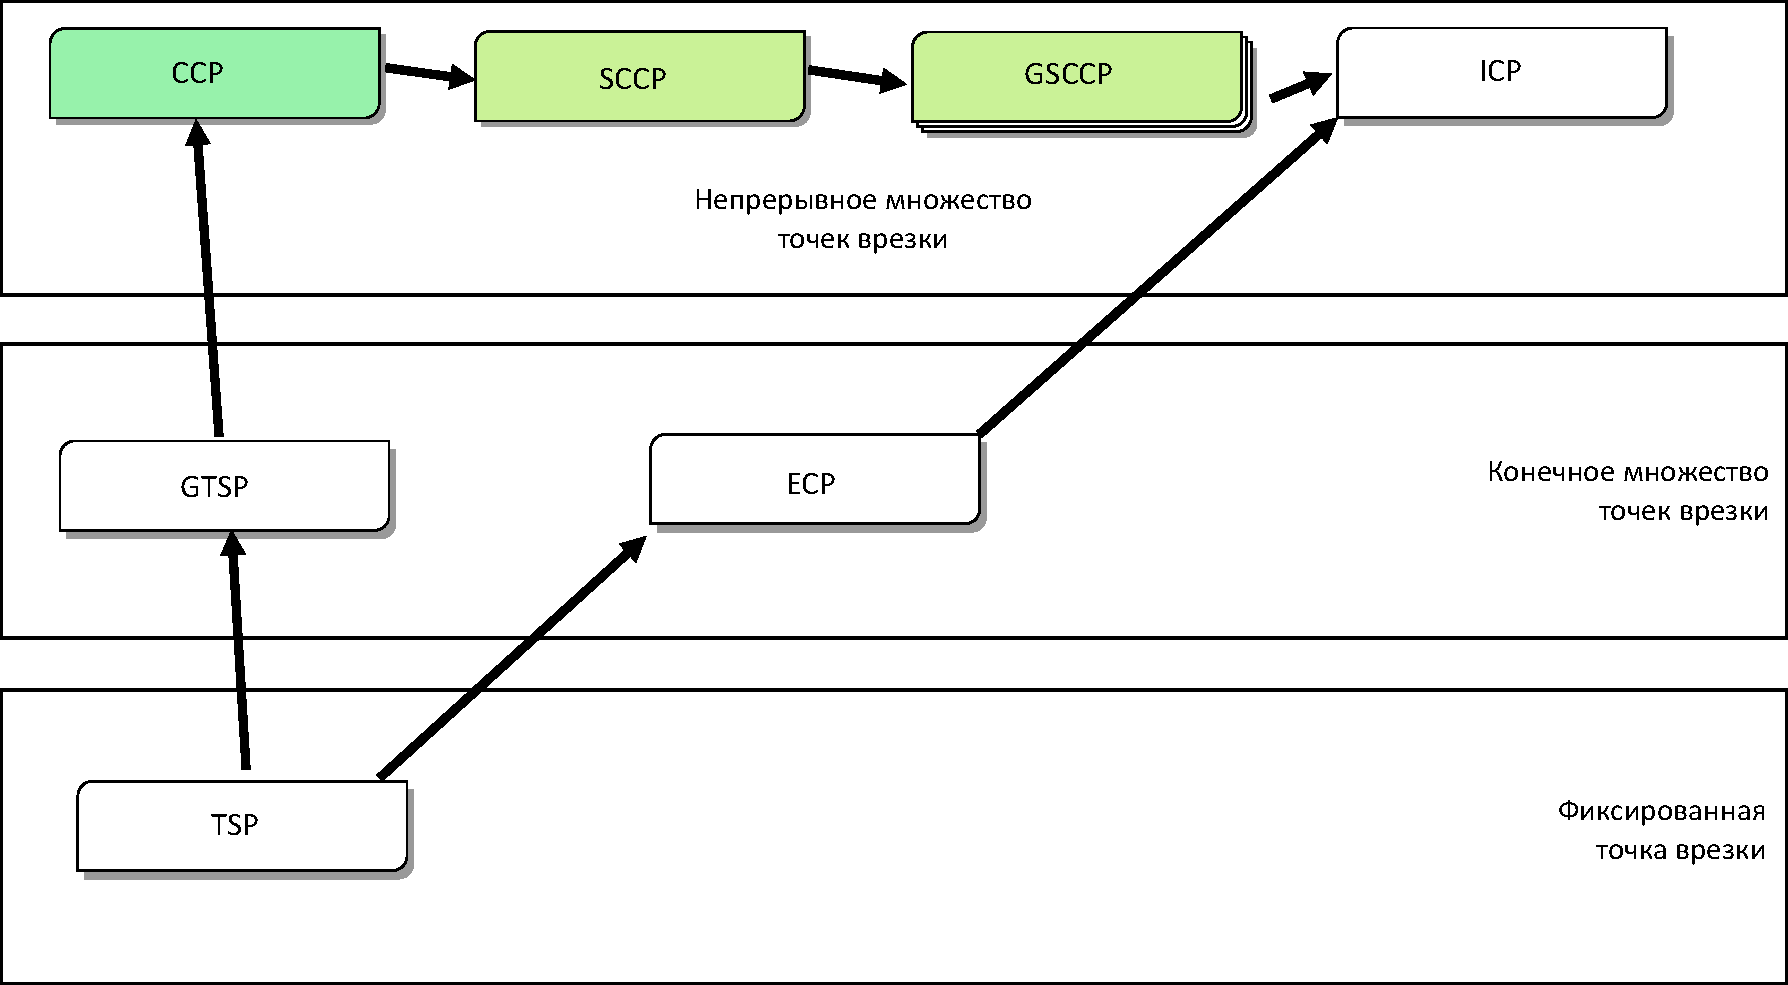
\includegraphics[width=0.95\textwidth]{classes.pdf}
  \caption{Классификация задач резки}
  \label{fig:cut-classes}
\end{figure}

В подавляющем большинстве исследований
непрерывно-дискретная
задача маршрутизации режущего инструмента~\eqref{eq:cut.problem}
как правило сводится
к задаче только дискретной оптимизации.
Для этого непрерывный контур детали
заменяется на конечное число
потенциальных точек врезки,
как правило расположенных на нём
с некоторым шагом
$\varepsilon$,
с учётом условия~\eqref{eq:cut.pierce},
то есть фактически сводится к
ECP
\cite{bi:Dewil2014,bi:Sherif2014,bi:Imahori2008}
или её частному случаю ---
GTSP
\cite{bi:Chentsov2018,bi:Petunin2017Apr,bi:Ye2013,bi:Yu}.
В этом случае,
полная ошибка в расчёте длины маршрута резки
составляет
$N \cdot \varepsilon$,
где
$N$
-- количество контуров,
подлежащих резке.
С ростом количества контуров
(что актуально для современного производства),
растёт и ошибка,
и для того,
чтобы гарантировать точность
$\delta$,
необходимо выбирать малый шаг дискретизации
$\varepsilon \approx \delta / N$,
в результате чего
общее количество точек на контурах растёт
($\sim O (N)$)
и время полного перебора также растёт,
но уже экспоненциально.
Тем не менее,
существуют изощрённые эвристики
решения таких задач даже для больших размерностей
~\cite{bi:RoMa}.
Использование непрерывной оптимизации,
без предварительной дискретизации ---
сравнительно мало исследованная область,
см. например~\cite{bi:Arkin1994,bi:Vicencio}.
